\documentclass[class=scrartcl, crop=false,parskip=half,]{standalone}
\usepackage[subpreambles=true]{standalone}
\usepackage{preamble}
\usepackage{import}
\usepackage{tikz}
\usepackage{tabu}


\begin{document}

\tikzset{
    sunflames/.style={
        line width=1pt,
        draw=red,
        fill=yellow,
        regular polygon, 
        regular polygon sides=3,
        inner sep=.05cm
    },
    sunbody/.style={
        line width=1pt,
        draw=red,
        fill=yellow,
        circle,
        minimum size=0.9cm,
    }
 }
 
%\section{The Sun}
The Sun is the central point of our solar system. It is about 5 billion years old and will persist in its current form about another 5 billion years before it becomes a red giant, expands and consumes the earth.

\begin{table}[ht] \label{tab:SunEarthData}
\caption{Data for the Sun and the Earth}
    \begin{tabular}{l l l l l}
    \hline\\
     & 	\textbf{Unit} & 	\textbf{Sun} & 	\textbf{Earth} & 	\textbf{Ratio (Earth: Sun)}\\
    \hline\\
    Radius & 	km & 	\num{6.97e5} & 	\num{6.38e3} & 	1:109\\
     \hline\\
    Diameter & 	km & 	\num{1.39e7} & 	\num{1.286e4} & 	1:109\\
    \hline\\
    Circumference & 	km & 	\num{4.37e6} & 	\num{4.0e4} & 	1:109\\
     \hline\\
    Surface area & 	\si{\km\squared} & 	\num{6.09e12} & 	\num{5.12e8} & 	1:11,900\\
    \hline\\
    Volume & 	\si{\km\cubed} & 	\num{1.41e18} & 	\num{1.08e12} & 	1:1,303,67\\
     \hline\\
    Mass & 	kg & 	\num{1.99e30} & 	\num{5.97e24}	&\\
    \hline\\
    Average density & \si{\kg\per\meter\cubed} & 	1,409 & 	5,516 & 	1:0.26\\
    \hline\\
    Surface gravity & 	\si{\newton\per\kg} & 	274 & 	9.81 & 	1:28\\
    \hline\\
    Surface temperature & 	K & 	5,777 & 	288 & 	1:367\\
    \hline\\
    Centre temperature & 	K & 	15,000,000 & 	6,700 & 	1:2,200\\
    \hline\\
    \end{tabular}
\end{table}


The sun consists of about 80\% hydrogen, 20\% helium and less than 0.1\% other elements.

In the sun, as in all stars of its type, \textbf{fusion} reactions occur as hydrogen nuclei (protons) fuse to form helium nuclei, each of which comprises two protons and two neutrons. These helium nuclei have a lower mass than the sum of the masses of the four protons required to form each one. This mass difference implies a release of energy with each fusion reaction, and it is this energy that is the electromagnetic radiation that emanates from the sun. The sun loses about 4.3 million tonnes of mass per second. The \textbf{solar radiant power} $\phi$ (the energy given out as electromagnetic radiation per second) is thus found, using Einstein's famous equation $E=mc^2$, where $c$ is the speed of light, to be


\begin{equation}\label{eq:solarRadiantPower}
    \phi_\mathrm{S}=\Delta mc^2=\num{4.3e9}\times\left(\num{3e8}\right)^2=\SI{3.845e26}{\watt}
\end{equation}

if this is divided by the surface area of the sun $A_\text{S}$, we find the specific emission $M_\text{S}$ of the sun which is the radiant power per square metre of the sun's surface:

\begin{equation}\label{eq:specificEmission}
    M_{\text{e,S}}=\frac{\phi_{\text{S}}}{A_{\text{S}}}=\SI{63.11}{\mega\watt\per\metre\squared}
\end{equation}

This means that every square metre of the sun's surface emits a  radiant power of 63.1 MW. That means that it takes only a fifth of a square kilometre of the Sun's surface to emit in one year an energy of 400 EJ, or 8700 Mtoe, which is currently the annual primary energy requirement of the earth's human population.% (IEA, 2013).


The sun's irradiance can be approximated to that of a \textbf{black body}. This is a perfect emitter, something that absorbs all radiation incident upon it then reemits it. Something black, like soot, is a good approximation to this. The spectrum of such an emitter was thoroughly investigated by various theorists and experimentalists in the latter half of the 19th century. Stefan and Boltzmann showed that the specific emission (total power emitted per square metre of surface) of a black body is proportional to the fourth power of the surface temperature, as :
\begin{equation}\label{eq:StefanBoltzmann}
    M_e(T)=\sigma T^4 \qquad \sigma=\SI{5.67e-8}{\watt\per\metre\squared\per\kelvin\tothe{4}}
\end{equation}
Since we know the specific emission of the sun, we can use equation \eqref{eq:StefanBoltzmann} to estimate the surface temperature of the sun:
\begin{equation}
    T_{\text{sun}}=\sqrt[4]{\frac{M_{\text{e,S}}}{\sigma}}=\SI{5777}{\kelvin}
\label{eq:Tsun}
\end{equation}
Wein showed that as the temperature of the surface of a black body varies, so does the frequency $f_\text{max}$ at which the emitted radiation is most intense. In fact, this frequency was found to be proportional to the surface temperature:
\begin{equation} \label{eq:WeinDisplacement}
f_\text{max}\propto T
\end{equation}
This upward shift in $f_\text{max}$ (and hence \emph{downward} shift in the wavelength $\lambda_\text{max}$ of the most intensely emitted radiation) with rising temperature should be familiar to you: when a metal rod is heated it first glows deep red - the lowest frequency/highest wavelength visible colour, then as it gets hotter it glows orange, then yellow, then finally blue, if heated to \SI{10000}{K}, at which temperature the most intense emitted radiation is actually in the ultraviolet. As it gets hotter, the dominant frequency increases and the dominant wavelength decreases.

As for the whole of the spectrum, this was observed experimentally by various workers and found to have the shape shown in Figure \ref{fig:bb_spectra} for two sources, one at 1000 K and one at 2000 K. The area under these curves is the total power emitted by each per square metre of surface. The hotter body emits far more power than the colder body - it shines more brightly.
\begin{figure}
\centering
\includegraphics[width=0.8\textwidth]{../figures/PlanckRadiation.tex}
\caption{The emission spectra of two black bodies - one at 2000 K and one at 1000 K. The vertical axis shows the intensity of the radiation at a particular radiation, while the total area under each curve show the total power emitted by the body - the greater the area, the more brightly the body shines. Notice that the hotter body shines more brightly and that the most intensely emitted radiation has shifted to lower wavelength, compared to the colder body}
\label{fig:bb_spectra}
\end{figure}
In a remarkable breakthrough in 1900, Planck was able account very precisely for these observations, but to do so he had to assume that light consisted of packets of energy, which we now know as photons. Black body spectra are widely observed in nature and the model of light as a stream of photons is crucial to an understanding of how photovoltaic cells work.

The solar radiant power spreads out uniformly in all directions, and by the time it reaches the earth it is spread over the surface of a sphere whose radius is the distance of the earth from the sun. This value varies since the earth follows an elliptical orbit about the sun, but its average value is about $r_\text{{se}}=\SI{1.5e11}{\metre}$. The surface of the sphere with this radius has area 
\begin{equation}\label{earthsSphereRadius}
A_\text{{se}}=4\pi r_\text{{se}}^2 = \SI{2.83e23}{\m\squared}
\end{equation}
and so the average value $E_0$ of the intensity of this radiation on reaching the top of the earth's atmosphere is
\begin{equation}\label{SolarConstant}
E_0=\frac{\phi}{A_\text{{s,e}}}=\frac{\num{3.845e26}}{\num{2.83e23}} =\SI{1367}{\watt\per\metre\squared}
\end{equation}
$E_0$ is known as the \textbf{solar constant}. It is an \textbf{irradiance} since it is a power per unit area, with units \si{\watt\per\metre\squared} and is measured at the top of the earth's atmosphere on a surface perpendicular to the radiation. Because of the variation in the sun-earth distance, mentioned earlier, the actual solar irradiance at the top of the atmosphere varies as the year goes by between about \SI{1325}{\watt\per\metre\squared} and \SI{1420}{\watt\per\metre\squared}.

Figure \ref{fig:SolarSpectra} show shaded in grey the spectrum of the sun on reaching the earth, before it enters the atmosphere, with a black-body spectrum for a source at 5700 K drawn on it. We that the two are very similar. The solar constant $E_0$ referred to above is the area shaded grey.

\begin{figure}
\centering
\includegraphics[width=0.8\textwidth]{../figures/SolarRadiation.tex}
\caption{A Planck radiation spectrum for a source at 5700 K, and solar spectra at AM0 and AM1.5}
\label{fig:SolarSpectra}
\end{figure}

From a solar energy point of view, more interesting is the curve shaded yellow, labelled as "AM1.5". This is the spectrum of sunlight once it has passed through the atmosphere to the earth's surface, where we can make use of it. This is our solar resource! Of great interest to us is the total irradiance, which is the area under the curve, and  how much of this irradiance comes from which range of wavelengths. We explore this in the next section.

\section{Solar Irradiance on the surface of the earth}
If we look at the AM1.5 spectrum in Figure \ref{fig:SolarSpectra} it is clear that the solar irradiance at the surface of the earth is lower than the solar constant, and that some wavelengths have been almost completely removed. This is because the atmosphere affects the radiation in various ways. These are
\begin{itemize}
\item reflection from the atmosphere
\item absorption by gas molecules in the atmosphere that contain three or more atoms, notably \ce{O3}, \ce{H2O} and \ce{CO2}. This absorption happens at particular wavelengths only, where the photon energy matches the energy difference between allowed states in the molecules. This accounts for the big dips in the terrestrial spectrum at some wavelengths.
\item \textbf{Mie} scattering - from water droplets, dust particles and other objects that are far larger than the wavelengths of light. All wavelengths that satisfy this criterion (which means all UV, all visible, all IR - everything that is cxoming fom the sun) are scattered with equal probability.
\item \textbf{Rayleigh} scattering - from molecules in the atmosphere, which all have a diameter much smaller than the wavelength of light. The probability of scattering from these sites is proportional to the fourth power of the light frequency. Blue light has roughly twice the frequency of red light and so is about $2^4=16$ times more likely to be scattered than red light. This is why the sky is blue! Sunlight that arrives in your eye from any direction other than that of the sun has been scattered, and hence is much more likely to be blue than red. 
\end{itemize}

The impact of these various factors depends on how much atmosphere the sunlight passes through before striking the ground, and on the cloudiness and pollution levels of that atmosphere.    \cite{SolarPositionCalculator}.

\subsection{Height of the sun in the sky and Air Mass}
The height of the sun in the sky will determine the total irradiance of the sun light when it reaches the ground, and also its spectrum, since Rayleigh scattering is frequency selective. An air mass or "AM" number is used to denote the spectrum of sunlight that arrives from a particular direction, having passed through a number of atmospheric thicknesses on the way. Light from directly overhead gives the AM1 spectrum, since it has passed through one atmospheric thickness, while light from any other direction will have passed through multiples of the atmospheric thickness, and so will be denoted by a higher AM number. the spectrum of ight at the top of the atmosphere, where it has not yet been attenuated by any air, is denoted by AM0.

The AM1.5 spectrum is particularly important, since this is the standard spectrum under which solar PV panels are tested and compared. It is the spectrum for sunlight that has passed through 1.5 atmospheric thicknesses.

The spectrum of sunlight arriving at the top edge of the atmosphere, just before it enters, is denoted AM0.

Both the AM0 and AM1.5 spectra are shown in Figure \ref{fig:SolarSpectra}.

Before going further, it is useful to introduce some terminology that is  used to describe the position of the sun in the sky.
\begin{itemize}
\item The \textbf{zenith} direction. This is the direction straight up from the ground.
\item The \textbf{zenith angle}. This is the angle between the zenith and a line drawn to the sun in the sky. This is \SI{0}{\degree} when the sun is directly overhead, and \SI{90}{\degree} when the sun is at the horizon.
\item The \textbf{solar height or altitude angle} $\gamma$ is the angle between the ground and a line drawn to the sun in the sky. This is \SI{90}{\degree} when the sun is directly overhead, and \SI{0}{\degree} when it is at the horizon.
\end{itemize}



\begin{figure}
\centering
\includegraphics[width=\textwidth]{../figures/airmass.tex}
\caption{Depending on where the sun is in the sky, its light will pass through different multiples of the thickness of the atmosphere before it reaches the ground. The longer this path becomes, the less intense the light on striking the ground and the more its spectrum is altered, as frequency dependent scattering and absorption occurs. A common way to denote the path length is in terms of "Air Mass" or AM number. the spectrum of light from when the sun is directly overhead is said to be AM1 by the time it reaches the ground- by then it has passed through one multiple of the atmosphere thickness, light striking the top of the atmosphere is AM0 - it has not yet passed through any atmosphere, while the spectrum light striking from any other angle has an AM number higher than one.The lower the sun is in the sky, the higher the AM number.}
\label{fig:airmass}
\end{figure}

The sun height angle $\gamma$ and the air mass number are approximately related by
\begin{equation}
\text{Air\ Mass\ Number} = \dfrac{1}{\sin \gamma }
\label {eq:AMnumber}
\end{equation}

The highest solar elevation reached at a location depends on the time of day,  the time of year and the latitude of the location. The nearer the time is to midday, the nearer the date is to midsummer, and the closer the location is to the equator, the higher the solar elevation will generally be. The precise variation with time of year and time of day depends on the latitude, however.

The higher the solar elevation, the lower the air mass and so the greater the irradiance at the surface of the earth. In regions at high latitude, the maximum solar elevation is much less in winter than in summer, and so in these regions the solar irradiance at the surface of the earth will also be less in winter than in summer, while in tropical regions, where there is little change in the maximum solar elevation from time of year to the next, the solar irradiance remains much more constant throughout the year.

Table \ref{tab:SolarReductionEffects} below shows the extent to which absorption, Rayleigh and Mei scattering can reduce the irradiation received at the surface of the earth for different sun elevations 

\begin{table}[ht] 
\caption{Solar radiation reduction influences at different sun heights. Note the general increase in reduction with air mass number, but note the very wide range there can be for any given sun height. This reflects local differences of clouds, weather and pollution between locations.}
\centering
    \begin{tabu}to 0.9\textwidth {  X[c]  X[c]  X[c] X[c] X[c] X[c] }
    \hline\\
    Sun Height  & Air Mass  & Absorption  & Rayleigh Scattering  & Mie Scattering  & Total Reduction\\  
    $\gamma_\text{S}$ & AM & (\%) & (\%) & (\%) & (\%)\\
    \hline\\
    \SI{90}{\degree} & 1.00 & 8.7 & 9.4 & 0 - 25.6 & 17.3 - 38.5 \\
     \hline\\
     \SI{60}{\degree} &1.15&9.2&10.5&0.7-29.5&19.4-42.8\\
    \hline\\
    \SI{30}{\degree} &2.00&11.2&16.3&4.1-44.9&28.8-59.1\\
     \hline\\
     \SI{10}{\degree} &5.76&16.2&31.9&15.4-74.3&51.8-85.4\\
    \hline\\
    \SI{5}{\degree} &11.5&19.5&42.5&24.6-86.5&65.1-93.8\\
    \hline\\
    \end{tabu}
\label{tab:SolarReductionEffects}
\end{table}

Apart from sun height, the irradiation over a day at a location depends on clouds, weather and pollution. The daily solar irradiation varies little throughout the year in equatorial regions, but the difference between summer and winter irradiation values increases as the latitude increases, in each hemisphere. There can also be great differences in daily irradiation between locations at similar latitudes, on account of differences in weather, cloud cover and pollution, but even more so between locations at different latitudes.


\end{document}

\begin{figure}
\centering
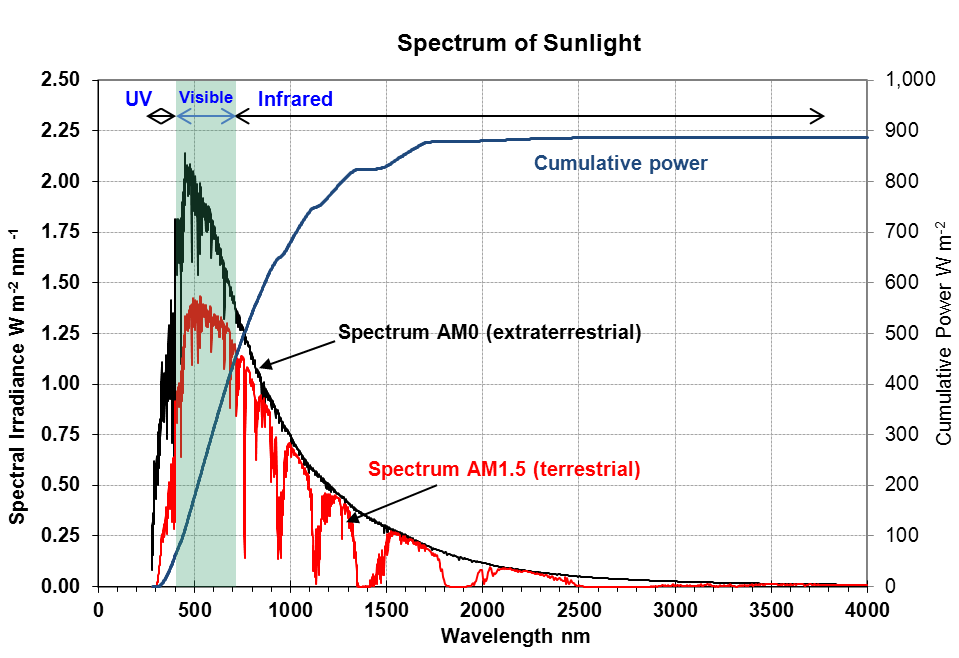
\includegraphics[width=\textwidth]{../figures/Reference_Spectra_ASTMG173.png}
\caption{Caption}
\label{fig:ASTMG173}
\end{figure}


